\chapter{Quoridor: Game description}
\label{GameDescription}

Quoridor is a 2, or 4 player game played in an NxN chess-like board where each player has a pawn and a set number of walls, where, typically the dimension of N is an odd number with 9x9 board being the most popular. In the game, each square represents a potential position for the pawn pieces. The board also contains grooves bordering each squares on the board where the player can place the walls. With 9x9 board, the total number of walls available to the player is 10.

The game starts with the pawn pieces of the players on the opposite side of the NxN square board. The starting position of the pawn is the center of the edge of the board associated with the side of the player. Each player, additionally, can place a wall on the grooves of the board between any two squares. The main objective is to be the first player to traverse with the pawn through the board to any one of the N squares on the opposite edge of the board. A player, in their each move, can either move a pawn or place a wall. The idea is that placing the wall between the squares means that the opponent cannot pass through the squares and potentially many need to take a longer route to reach the opposite edge of the board. Hence, the strategy of a player in the game is to be the first player to move
their pawn to the row of squares on the opposite edge of the game board avoiding any walls deterring its path to the goal while strategically placing walls to deter opponents from reaching their goal squares.

The Quoridor game is played in turns between the opponents where in each turn the player can either move a pawn or place a wall. Then the move shifts to the opponent player(s) where they can do the same in their turn.

Walls are a fundamental element of the game, allowing players to strategically block their opponent's path and influence the course of the game. Each wall spans across two squares on the board and occupies exactly four squares either horizontally or vertically, effectively creating a barrier between them. At the beginning, each player starts
with a set number of walls that they can use during their turn.

\begin{figure}[!ht]
    \centering
    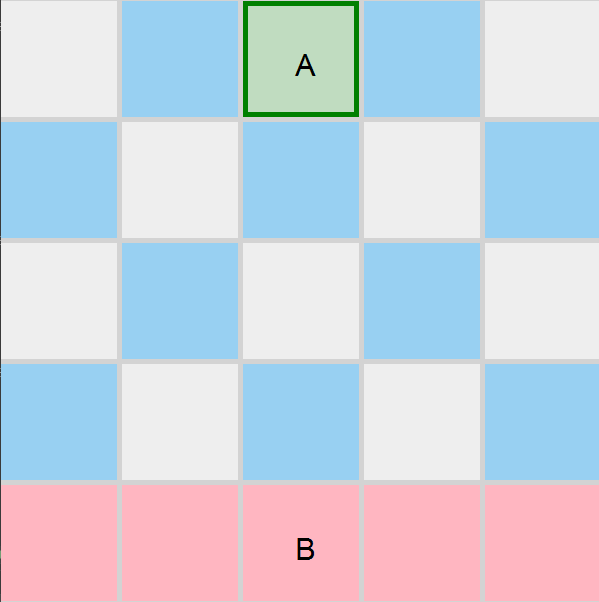
\includegraphics[scale=0.25]{../img/GameBoard/initial.png}
    \caption{A screenshot of a 5x5 game board from our implementation}
    \label{fig:InitialGameBoard}
\end{figure}

As seen in Figure \ref{fig:InitialGameBoard}, in this thesis, we consider a two-player Quoridor game with player A and player B. The pawn of player A is represented by the letter 'A' and that of player B is represented by the letter 'B'. In the figure, we display a 5x5 board with the squares on the edge of the board highlighted in pink belonging to player B whereas the squares on the opposite edge of the board belonging to player A. The board in the figure also shows the starting position of the two players with the pawn at the center of their respective edges. The goal of player A is to move its pawn through the board to one of the squares on the edge belonging to player B that has been highlighted in pink. The gray areas between the squares on the board represents the grooves of the board where walls can be placed. As mentioned earlier, the length of the walls is equal to the length of two squares. Hence, placing a wall on the board touches four squares where two squares are on one side of the wall whereas the two other squares are on the opposite side of the wall. The player cannot cross the squares through the wall. 

In order to formalize the game, we have to define the notations and use it to formally define the game rules and the player movement and wall placement rules.

\section{Notation}

In this subsection, we will first consider the notations popular in the literature and the Quoridor community and then define our own notation, especially for the wall placement, while analyzing the differences between them. This definition of our own notation is motivation by the ambiguity that we present existing in the current notation.

There are no official notations for this game. However, some popular ones recognized by the Quoridor community
include \textbf{Glendenning's Notation} (\citep{Glendenning2002MasteringQ}) and the \textbf{Quoridor Strat's Notation}
(\citep{website:COMMUNITY_NOTATION}). We first consider the notations in these two references below:

First, defining the notation of the squares of the board, consider a Quoridor board of dimension 9x9 as an example. Let $\mathbb{K} = \{a, ..., i\}$ and $\mathbb{R} = \{1, ..., 9\}$ and $C$ denote the 2D Quoridor board with $C_{i,j}$ representing the $i$-th row and $j$-th column position of the cell. Both the Glendenning's and Quoridor Strat's notations follow the same principle of labelling each cell or a square by $C_{i,j}$ where $i \in \mathbb{R}$ and $j \in \mathbb{K}$. Hence, in this approach the board is labelled by a combination of alphabetical letters (e.g., $\mathbb{K}$) denoting the columns and the positive integers (e.g., $\mathbb{R}$) representing the rows. This follows the similar style of notation for labelling the squares in chess.

This notation can be extended to a Quoridor board of any dimension NxN by considering the dimension of both $\mathbb{K}$ and $\mathbb{R}$ as $N$ where $\mathbb{K}$ is the set of first $N$ alphabetical characters in an ascending order and $\mathbb{R}$ is the set of first $N$ positive integers in a ascending order.


Considering an example in Figure \ref{fig:InitialGameBoard}, with these notations, the pawn A is in the position $C_{1, c}$ and the pawn B is in the position $C_{5, c}$.

After representing the Quoridor board, the next step for defining notations for the game is to define the moves. Let us represent the move for a player as $M$.

\begin{equation}\label{eqn:movement}
M(C_{ij}) = ji \text{, where, } j \in \mathbb{K} \text{ and, } i \in \mathbb{R}     
\end{equation}

Unlike in chess, in Quoridor, there is only one pawn for each side. Hence, for the side, for moving the pawn, the starting position of the pawn is not required. Hence, as mention in Equation \eqref{eqn:movement}, the movement of the pawn to the cell $C_{j, i}$ can simply be defined by the notation $ji$. The movement of the pawn A, in Figure \ref{fig:InitialGameBoard} from its position from cell $C_{1, c}$ to the position of B in $C_{5,c}$ through the cells $C_{2, c}$, $C_{3, c}$ and $C_{4, c}$ can be defined with moves $c2$, $c3$, $c4$ and $c4$ requiring a total of 4 moves.

Additionally, as described earlier, the Quoridor game is played between multiple players where each player in a turn can make a move. Hence, the turns are represented numerically, for e.g., 1., 2., 3. represents the first, second and third move respectively. Hence considering the scenario where player A moves its pawn in Figure \ref{fig:InitialGameBoard} from $C_{1,c}$ to $C_{2,c}$ and then to $C_{3,c}$ and player B moves its pawn from $C_{5,c}$ to $C_{4,c}$ to $C_{4,b}$, the notations can be represented as: $1. C2 C4$, $2. C3 B4$. Here the numbers 1. and 2. represents the two moves of each players and $1. C2 c4$ represents the movement of the players A's pawn to C2 and then player B's pawn to C4. The order of the player's movement can be dependent on the player that moves first. For example, in the example, player A moves first to $C4$, hence it is notated before player B's move. This order has to remain constant throughout the game.

Similarly, after notation of the board and the movement, the notation for wall placement is another important component for Quoridor. The notation for wall placement is defined by the following equations:

\begin{equation}\label{eqn:wall1}
W(C_{i,j}) = jiD \text{ , where, } j \in \mathbb{K}, i \in \mathbb{R}  \text{ , and } D \in \{h, v\}
\end{equation}

In the above equations, the wall is represented with respect to a reference cell. In the above equation, the reference cell is $C_{i, j}$. As described earlier, the length of the wall is equivalent to the length of two cells. Hence, the reference point of the cell determines the starting point of the wall placement that covers two cell lengths. Likewise, $D$ in Equation \eqref{eqn:wall1} defines the arrangement of the wall. The wall from a reference point can be placed vertically or horizontally. This is represented in the equation by the characters 'h' and 'v' respectively.

In the notations defined as per Glendenning's notations and Quoridor Strat's notations, there is a difference when it comes to the wall representation even though the mathematical formulation is the same as presented in Equation \eqref{eqn:wall1}. 

\begin{figure}[!ht]
    \begin{subfigure}{0.4\textwidth}
      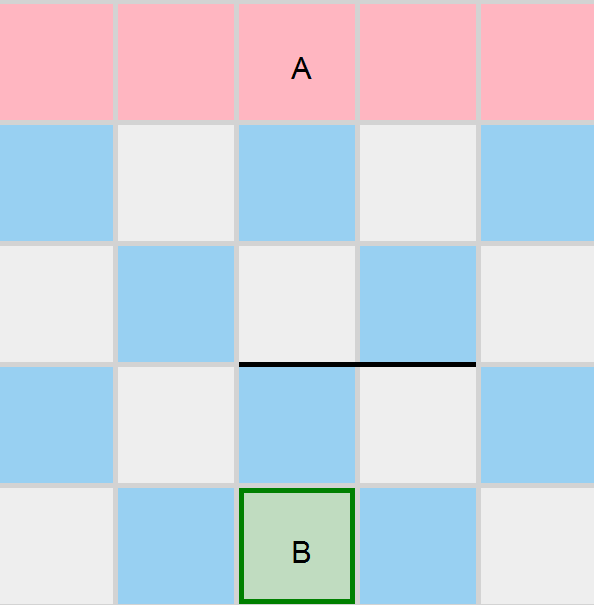
\includegraphics[width=\textwidth]{../img/GameBoard/wall_repr.png}
      \caption{Glendenning's Notation: \textbf{c3h}}
      \label{fig:NotationDifferentA}
    \end{subfigure}
    \hfill
    \begin{subfigure}{0.4\textwidth}
      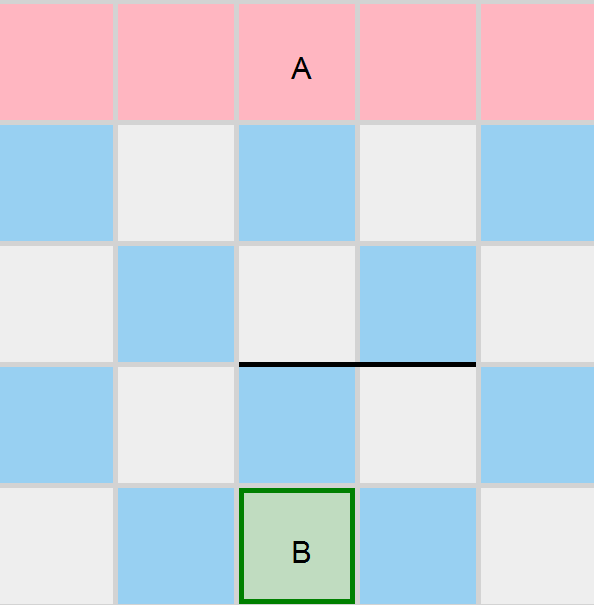
\includegraphics[width=\textwidth]{../img/GameBoard/wall_repr.png}
      \caption{Quoridor Strats Notation: \textbf{c4h}}
    \end{subfigure}
    \caption{Notation differences}
    \label{fig:WallNotationsDifferent}
\end{figure}

As seen in Figure \ref{fig:WallNotationsDifferent}, the difference lies in the exact position of the reference point of the walls of the wall. In the reference square, there are 4 corners. The reference point for horizontal wall placement is always the left corners of the cell. However, the difference in the notations lie in fact that whether the reference left corner is the left upper corner or the left lower corner. In the Quoridor Strats Notation, the reference starting point of the wall  is defined by the lower-left corner of the sqaure whereas in the Glendenning's Notation, each wall starts from the upper-left corner of the square. This difference is exemplified in the figure \ref{fig:WallNotationsDifferent}. In Glendenning's Notation, the wall placement with reference to the square $C_{3, c}$ i.e., c3h is defined with respect to the lower left corer of the square $C_{3. c}$. In contrary, in the Quoridor Strats Notation, the wall placement with reference to the $C_{4,c}$ i.e., c4h, is defined with respect to the upper left corner of the cell $C_{4,c}$. Since the lower left corner of the cell $C_{3,c}$ and the upper left corner of the cell $C_{4,c}$ are the same, the wall placement due to the notation difference were the same as seen in the figure.

Even though there notations are widely used, they are very easy to get confused with since they have the same wall representations,
and unless specified explicitly, it is difficult to tell which representation is being used. This ambiguity in notation necessitates a new notations, in particular for the wall placement to remove any confusion. For this purpose, in this thesis, we introduce a new notation for the purpose, particularly, of wall placement representation as follows:

\begin{equation}\label{eqn:Wall2}
W(C_{ij}) = jiD \text{ , where, } i \in \mathbb{R}, j \in \mathbb{K} \text{ ,and, } D \in \{N, S, E, W\}    
\end{equation}

In this new notation, we increase the size of the set $D$ from horizontal and vertical representation to north, south, east and west representations indicated by the characters 'N', 'S', 'E' and 'W'. This ensures that instead of an ambiguous vertical and horizontal wall representation with  respect to a cell, we can now define the direction explicitly. This wall additionally also implies that the wall in the 'N' and 'S' direction covers the reference cell, i.e., $C_{i, j}$ and the cell right to the reference cell, i.e., $C_{i, j+1}$ where $j+1$-th column represents the column on the right of the $j$-th column. Similarly, the wall in the 'E' and 'W' directions implies that the wall covers the reference cell $C_{i, j}$ and the cell below the reference cell, i.e., $C_{i+1, j}$ where $i+1$-row represents the row below the $i$-th row.

Looking back at Figure \ref{fig:NotationDifferentA}, the walls can now be represented by \textbf{c4N}, i.e. a Northern wall from the cell $C_{4, c}$.

This notation provides an additional flexibility to represent the wall placement in the game and removes the ambiguity that may be present as we saw earlier.

\section {Rules}
In this section, we formally define the rules of the game Quoridor, in particular for the wall placement and player movement.

\subsection{Wall placement rules}
\label{WallRules}

\begin{itemize}
    \item The walls have to be placed in either vertical or horizontal manner and they cannot be placed diagonally.
    \item A placed wall must not completely block any player's path to victory. Each player must have at least
        one path to victory. For example, in Figure \ref{fig:ValidState}, the walls are placed in such a way that player A has a valid path towards the edge of the player B, in particular, to the cells $C_{5, a}$, $C_{5, b}$, $C_{5, c}$, $C_{5, d}$ and $C_{5, e}$. However, the wall placement in Figure \ref{fig:WallBlockingMove}, due to the placement of the wall \textbf{c3N}, the player A does not have a valid path towards the edge cells of player B. Hence, the move \textbf{c3N} would be classified as an invalid move.
    \item A placed wall cannot intersect any of the previously placed walls. For example, in Figure \ref{fig:ValidState}, a walls has been placed with the moves \textbf{a1W}. A subsequent move \textbf{a2N} would be an invalid move in the game due as it requires the walls to intersect.
    \item Walls cannot be placed along the edges of the board. Walls must be placed to create a barrier for exactly 4 cells. For example, in Figure \ref{fig:ValidState}, a wall cannot be placed with the move \textbf{a1E} as it would only touch 2 cells $C_{1, a}$ and $C_{2, a}$ as it is on the edge of the board.
    \item  Every player possesses a limited supply of walls, and once they exhaust these walls, they are unable to place any additional ones. Consequently, in such situation the player is only allowed to maneuver their pawn on the
        board.
\end{itemize}

\begin{figure}[!ht]
    \begin{subfigure}{0.4\textwidth}
      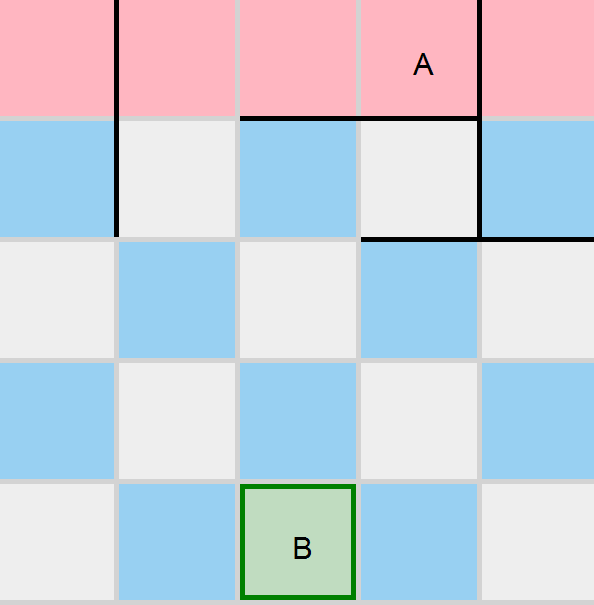
\includegraphics[width=\textwidth]{../img/GameBoard/arbitrary_state.png}
      \caption{Valid game state}
      \label{fig:ValidState}
    \end{subfigure}
    \hfill
    \begin{subfigure}{0.4\textwidth}
      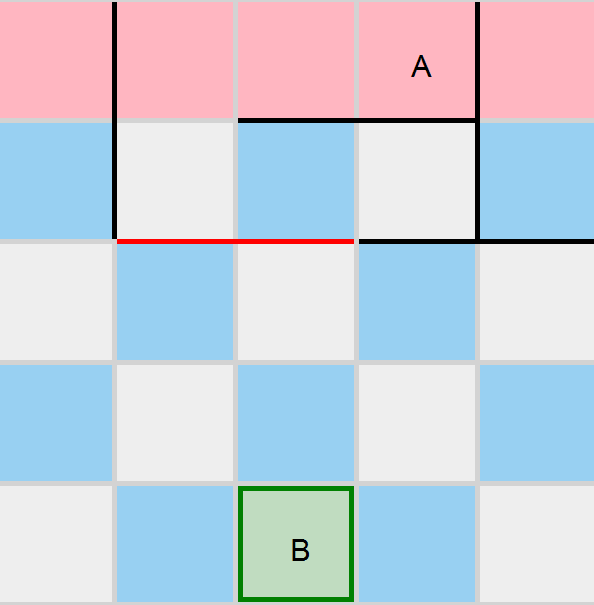
\includegraphics[width=\textwidth]{../img/GameBoard/invalid_wall.png}
      \caption{Invalid wall \textbf{b2S}}
      \label{fig:WallBlocked}
    \end{subfigure}
    \caption{Example of an invalid wall placement}
    \label{fig:WallBlockingMove}
\end{figure}

The game state represented by Figure \ref{fig:ValidState} shows the situation after 5 turns, with it currently
being player B's turn to move. Since both \textbf{A} and \textbf{B} have viable paths to their respective goal
rows and all walls have been placed according to the rules (see \textit{Section \ref{WallRules}}),
the game state shown in Figure \ref{fig:ValidState} is considered valid.
\par
However, player B disrupts the rules by placing the red wall, violating the specified wall-placement rules
(see \textit{Section \ref{WallRules}}), consequently rendering the game state represented by
Figure \ref{fig:WallBlocked} invalid.

\subsection{Player movement rules}
\label{PlayerMoveRules}
\begin{itemize}
    \item Players are allowed to move their pawn one cell at a time in the North, South, East, or West directions during their turn given that there is a cell and the cell is empty in the direction. Diagonal movements are not allowed. For example, a pawn in a cell $C_{2, c}$ can move to either in the north direction (i.e., $C_{1, c}$), the south direction (i.e., $C_{3, c}$), the west direction (i.e., $C_{2, d}$) or in the east direction $C_{2, b}$ given that the adjacent cells or squares empty. However, a pawn in the cell $C_{1,a}$ can only move in the west (i.e., $C_{1,b}$) and the south (i.e., $C_{2,a}$) direction as there are no squares on the east or the north of the cell.

    \item \textbf{Jump}
    \begin{itemize}
        \item If an opponent is at to the cell a player intends to move in the same direction of the opponent, the player can jump over the opponent provided there is no wall between the opponent or behind the opponent they intend to jump over. For example, in the first picture in figure \ref{fig:PossibleMoves} the player B can move to either of the squared highlighted in green. The player can move to east, west or south direction or can jump in the north direction over the player A from square $C_{4,c}$ to the square $C_{2,c}$ as there are no walls between the squares $C_{4,c}$, $C_{3,c}$ or $C_{2,c}$.
        
        \item If there is a wall between the opponent and the jumping square, the player can jump to a cell on either side of the opponent's cell, given the cell is accessible from the opponent's cell (i.e., there are no walls). In the section picture from left in the figure, for example, the player B cannot jump over player A to the cell $C_{2, c}$ due to the wall placement \textbf{c3N}. The player in this case can jump over to the cells on either the east side (i.e., cell $C_{3, b}$) or the west side (i.e., cell $C_{3, d}$) of the player A given there are no walls in between $C_{3, c}$ and $C_{3, b}$, and $C_{3, c}$ and $C_{3, d}$ respectively.
            
        \item Players cannot jump over walls. If a player is jumping from a cell $C_{1,*}$ to cell $C_{3,*}$, this is only possible if there are no walls in between them.
    \end{itemize}
\end{itemize}

\begin{figure}[!ht]
    \begin{subfigure}{0.2\textwidth}
      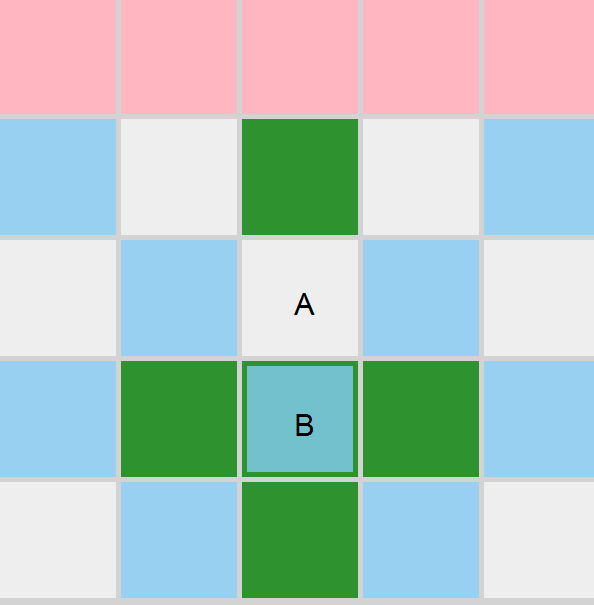
\includegraphics[width=\textwidth]{../img/GameBoard/move01.png}
    \end{subfigure}
    \hfill
    \begin{subfigure}{0.2\textwidth}
        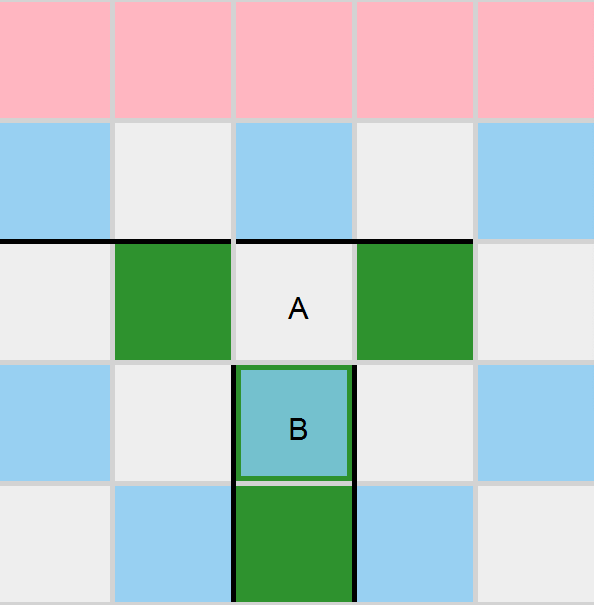
\includegraphics[width=\textwidth]{../img/GameBoard/move02.png}
    \end{subfigure}
    \hfill
    \begin{subfigure}{0.2\textwidth}
        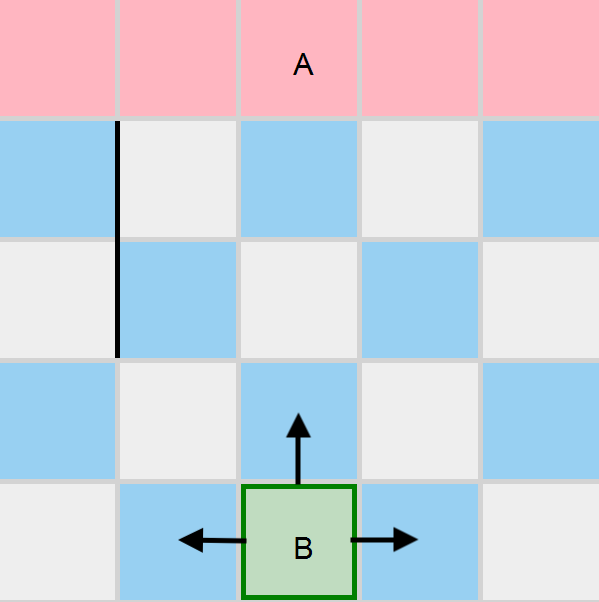
\includegraphics[width=\textwidth]{../img/GameBoard/move03.png}
    \end{subfigure}
    \hfill
    \begin{subfigure}{0.2\textwidth}
        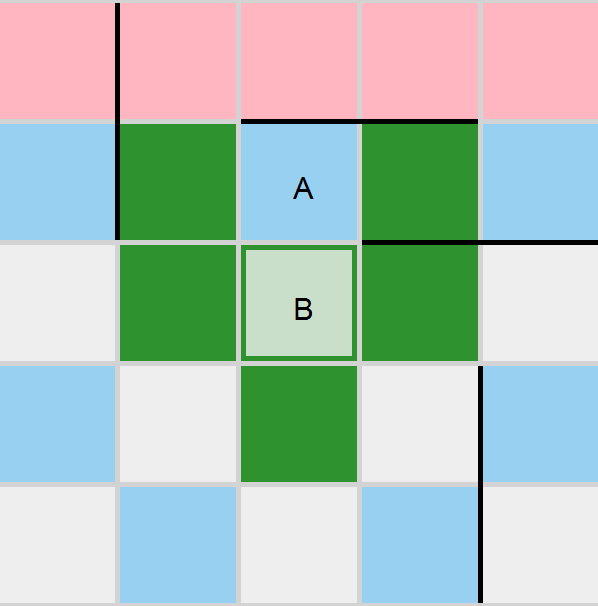
\includegraphics[width=\textwidth]{../img/GameBoard/move04.png}
    \end{subfigure}
    \caption{Examples of possible moves (marked green) for player B in different game states}
    \label{fig:PossibleMoves}
\end{figure}